% Created 2020-04-22 Wed 22:00
% Intended LaTeX compiler: pdflatex
\documentclass[11pt]{article}
\usepackage[utf8]{inputenc}
\usepackage[T1]{fontenc}
\usepackage{graphicx}
\usepackage{grffile}
\usepackage{longtable}
\usepackage{wrapfig}
\usepackage{rotating}
\usepackage[normalem]{ulem}
\usepackage{amsmath}
\usepackage{textcomp}
\usepackage{amssymb}
\usepackage{capt-of}
\usepackage{hyperref}
\usepackage{geometry}
\usepackage{charter}
\usepackage{booktabs}
\usepackage{float}
\author{fbi}
\date{\today}
\title{}
\hypersetup{
 pdfauthor={fbi},
 pdftitle={},
 pdfkeywords={},
 pdfsubject={},
 pdfcreator={Emacs 26.3 (Org mode 9.1.9)}, 
 pdflang={English}}
\begin{document}

\begin{titlepage}
   \begin{center}
       \vspace*{1cm}


        {\textbf{\Huge iDrop User Manual}}


   \end{center}
\end{titlepage}


\section{Description}
\label{sec:org0f9fa96}
The iDrop is a machine that generates rhythms using standard drum
sounds. The user can choose from a set of six instruments to play in a
sequence of twelve

beats (Beats are the basic timing unit used in music). Each beat can
play more than one instrument at a time. Once an instrument is chosen,
the user can choose which beat the instrument should play
on. Afterwards, the machine will be able to play back the sequence
with each beat updated for the chosen instrument. The machine will
infinitely loop through the sequence of twelve beats until it is
turned off.  This product is intended for those who wish to have a
basic understanding of music production using a drum kit. A drum kit
can create a rhythm using basic sounds. For six instruments and twelve
beats, there are many possibilities for rhythm patterns. On top of
that, the iDrop offers the ability to change the speed (BPM) with
which the sequence of twelve beats plays.  Much of this machine’s
design was completed before the COVID-19 lockdown, resulting in
limited access to facilities where a physical prototype could be
compiled. Thus, our product has been converted to a software medium in
which the original functions of the physical prototype can be
simulated. This manual will focus on the operation of the software
implementation of the iDrop.

\section{Guided Tour of iDrop}
\label{sec:org7dd0dad}
Below is a screenshot of the default iDrop application. Here no
instruments are being played. The pane to the left is called the
\emph{sequencer} and is where to create the drum pattern that forms your
beat. The drum loop is split into 16 \emph{beats} which are the times
when a instrument gets played. The sequencer scans from left-to-right
and loops back again and plays back instruments when they are actived.
The small dot under an active beat will turn light-gray on the beat
that the drum machine is current on. In the below example, the current
beat is the 3rd from the last. Below the labels for each instrument in
the sequencer are buttons that allow you to turn on and off each instrument
for each beat.

\begin{center}
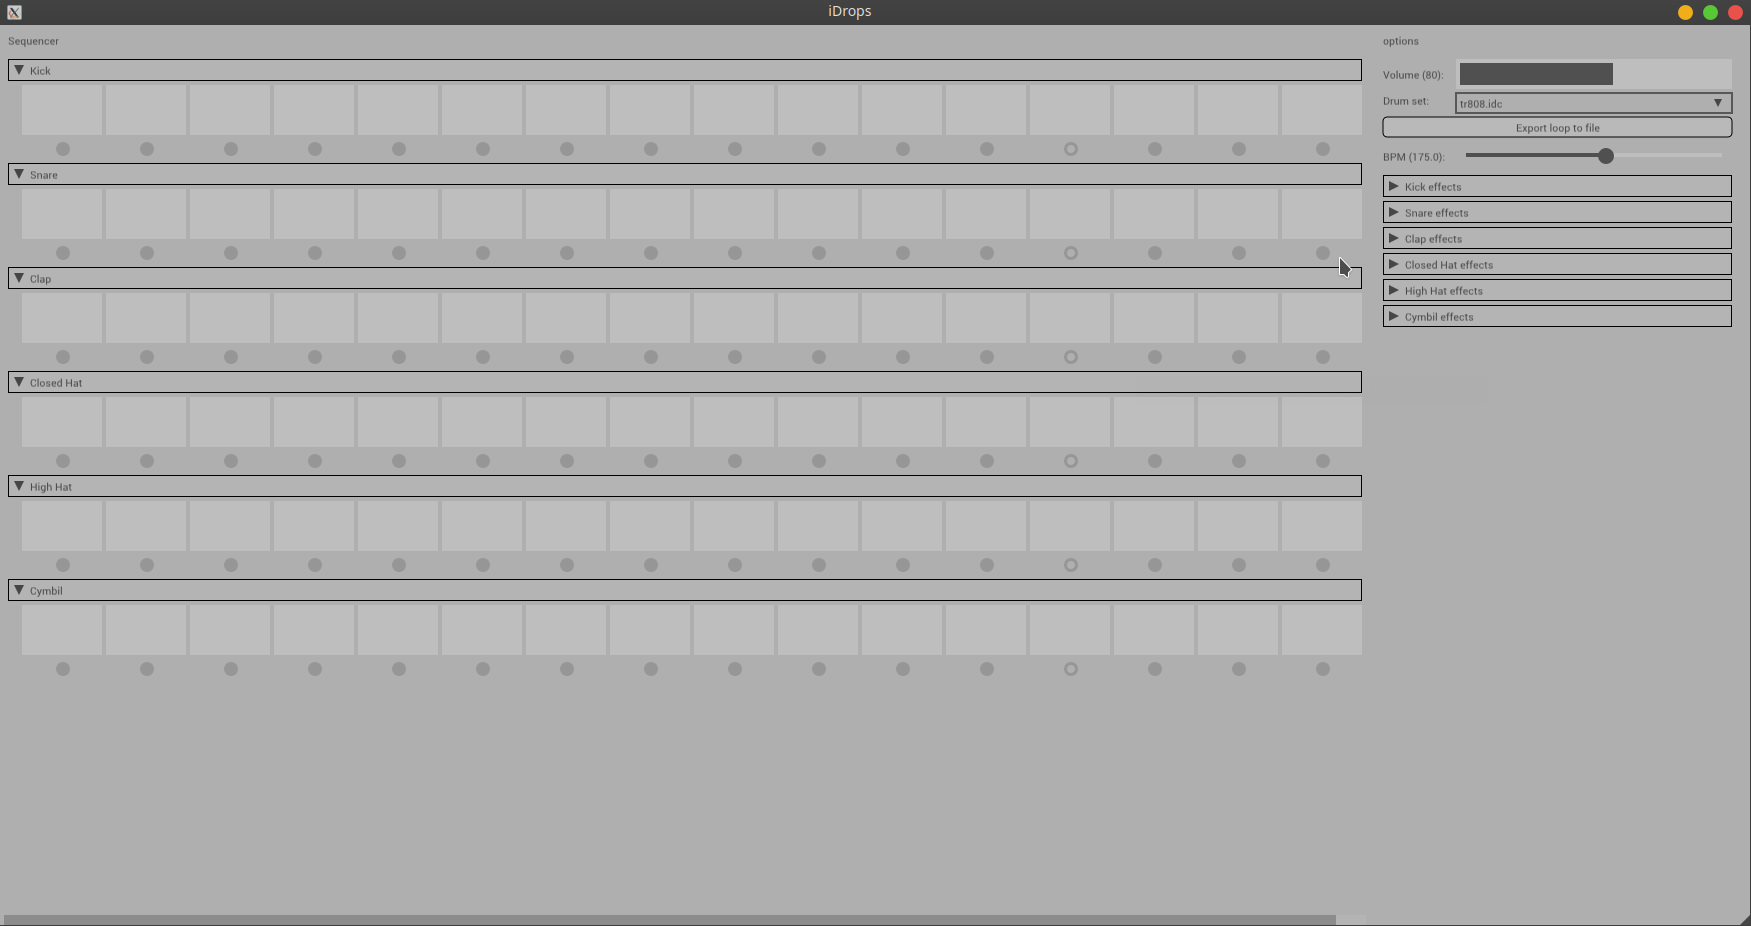
\includegraphics[width=15cm]{./default.png}
\end{center}

To turn on an instrument on a specific beat, click the large square
under the desired instrument and it will turn dark-gray indicating
that the instrument is now active on that beat. Click it again to turn
it light-gray and toggle the instrument off on the beat. The picture
below shows a screenshot with the "kick" drum turned on for some beats.

\begin{center}
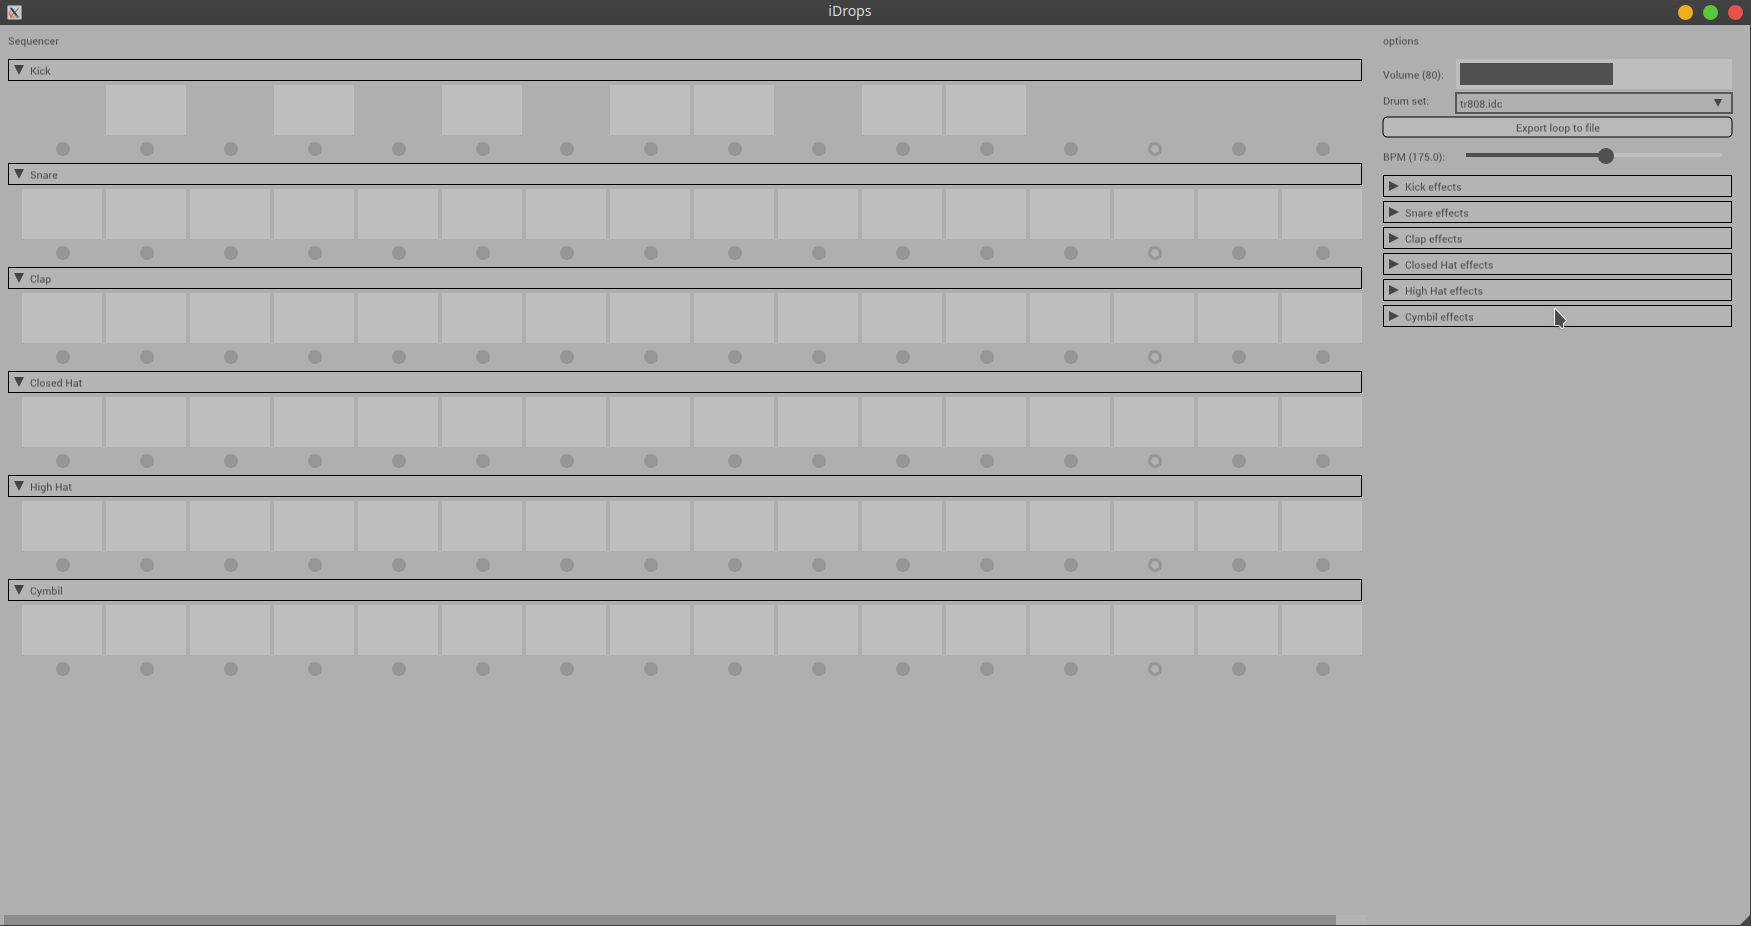
\includegraphics[width=15cm]{./no2.png}
\end{center}

Now you may want to start adjusting the options for your instrument. To
change the overall volume, use the "volume" slider in the options panel to
change the global volume of the application. If you would like to apply affects
to only one instrument, click on the label of the instrument you want to change
options for. The picture below shows a mouse hovering over the "kick effects".

\begin{center}
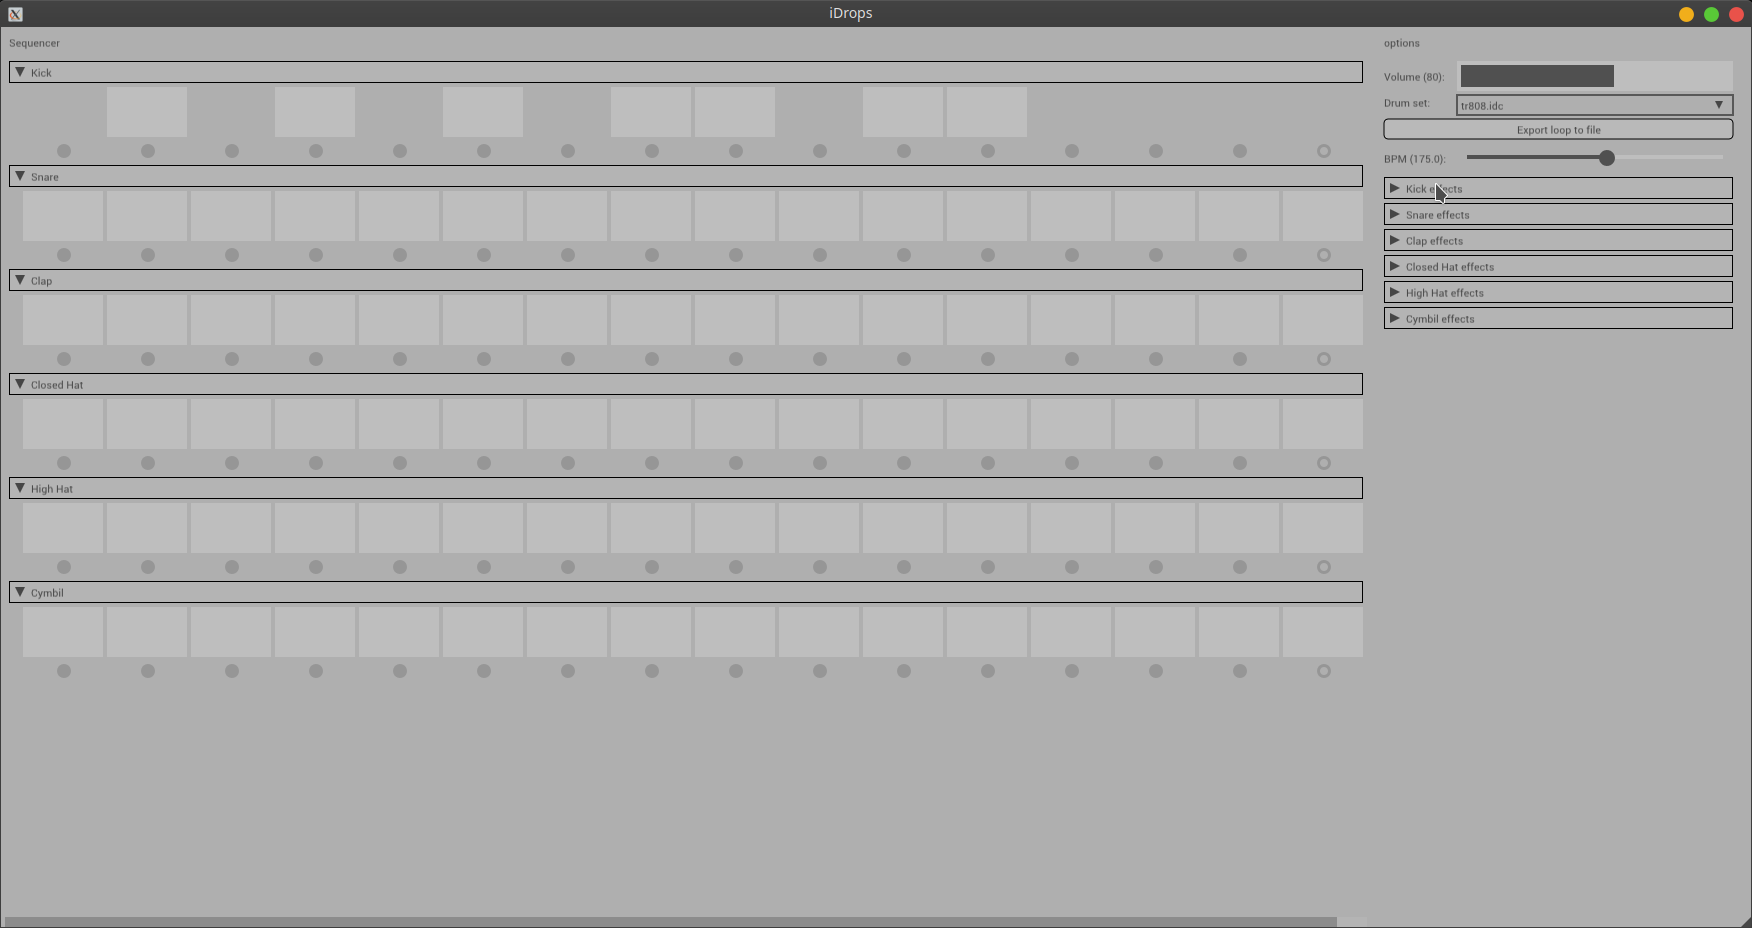
\includegraphics[width=15cm]{./3.png}
\end{center}

Now clicking the label opens up the menu for the instruments options.

\begin{center}
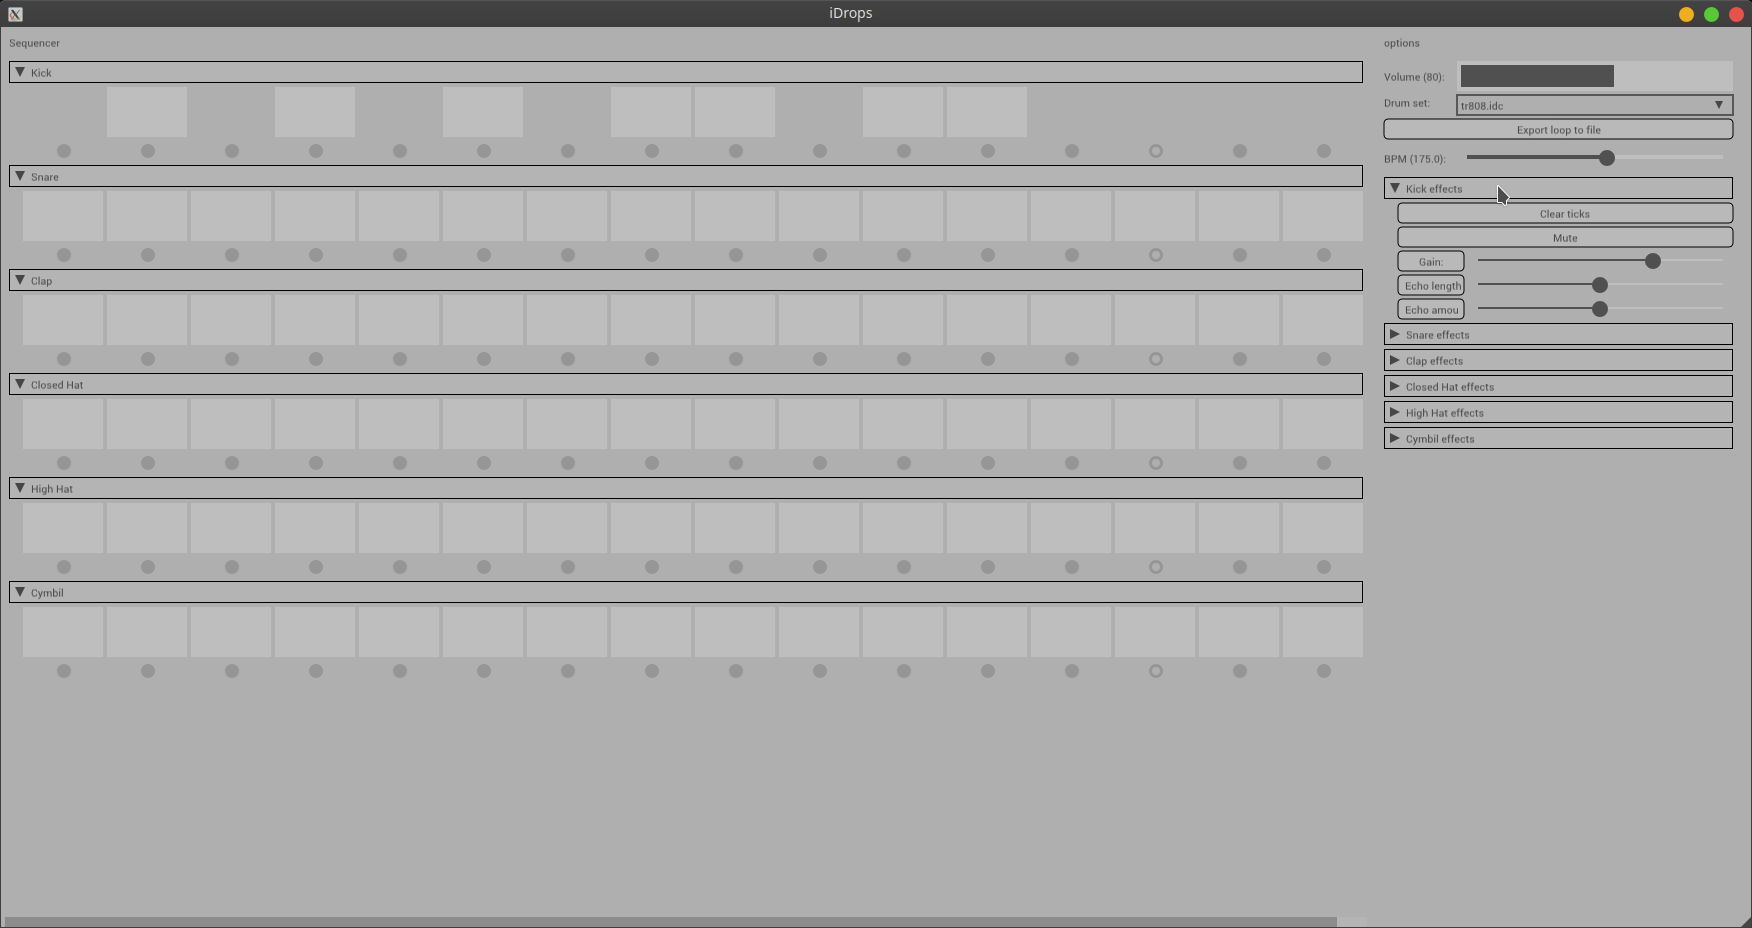
\includegraphics[width=15cm]{./4.png}
\end{center}

Under this menu you will find a few important options. The slider labeled "gain"
will allow you to adjust the instruments volume level without affecting the
volume of other instruments. The echo length slider allows you to delay when 
the echo effect occurs, while the echo amount changes how fast the echo decays.
A larger echo amount means the echo will decay faster. If you make a change to
these sliders and do not like it, simply press the labeled button to the left
to reset the effect to its default amount.

\begin{center}
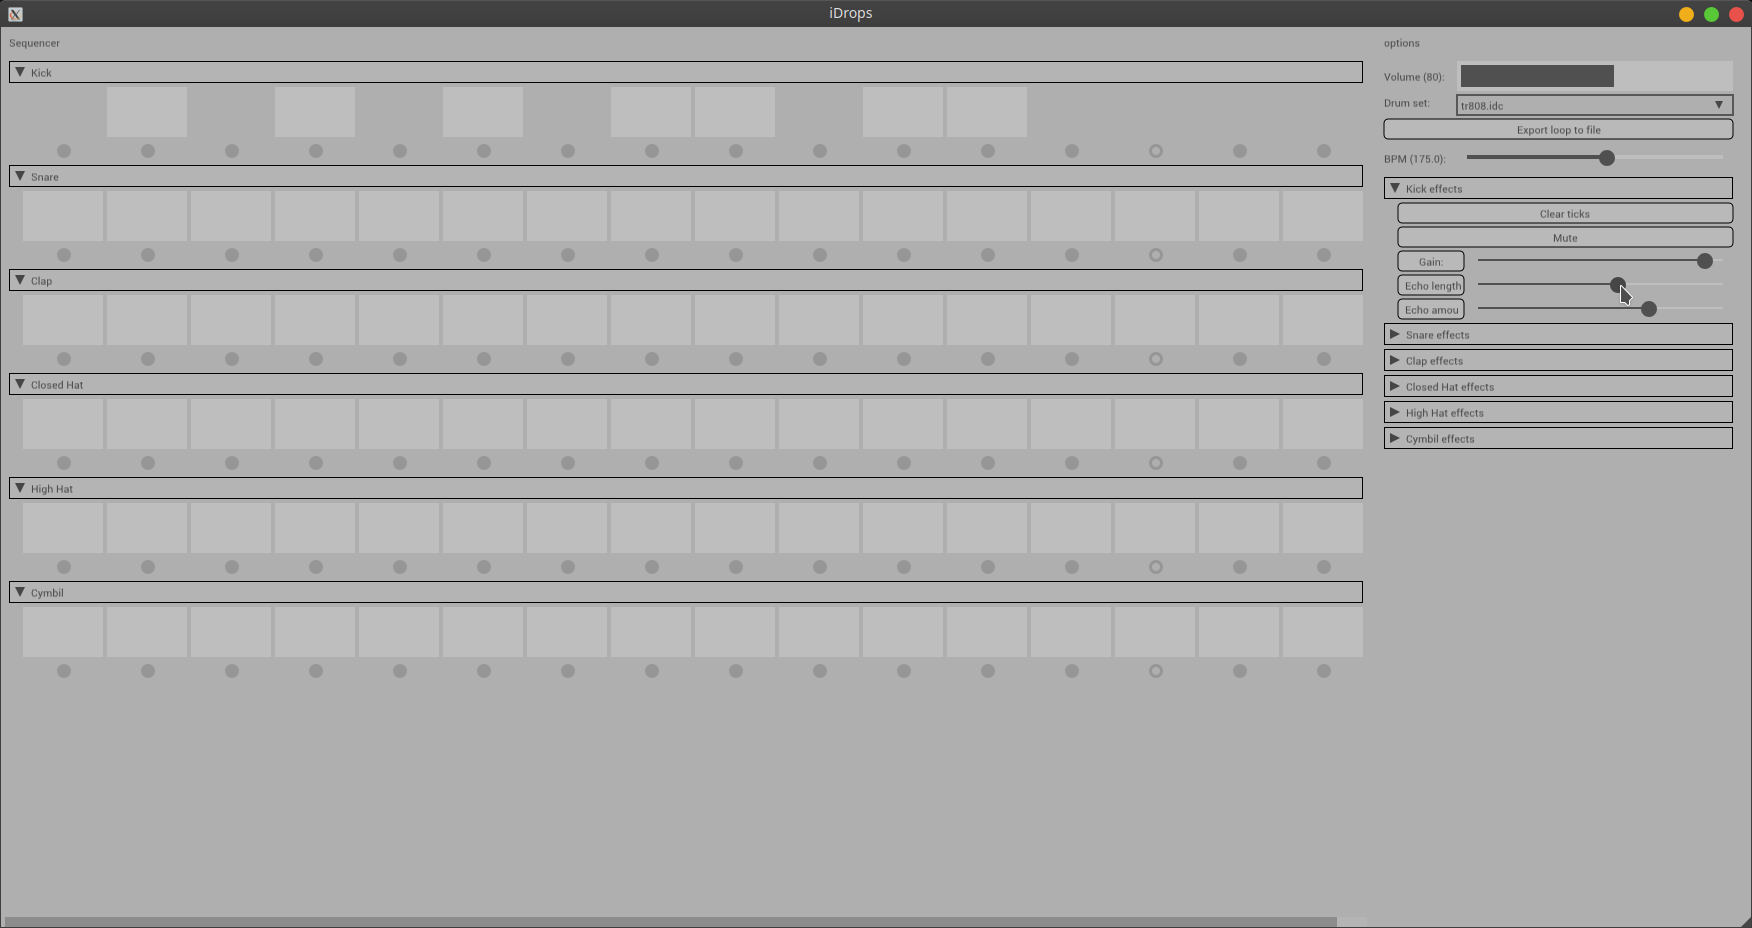
\includegraphics[width=15cm]{./5.png}
\end{center}

If you want to temporarily mute the instrument, click the buttoned labeled "mute".
If you would like to clear the pattern for the instrument, click the "clear ticks"
button as in the below picture.
\begin{center}
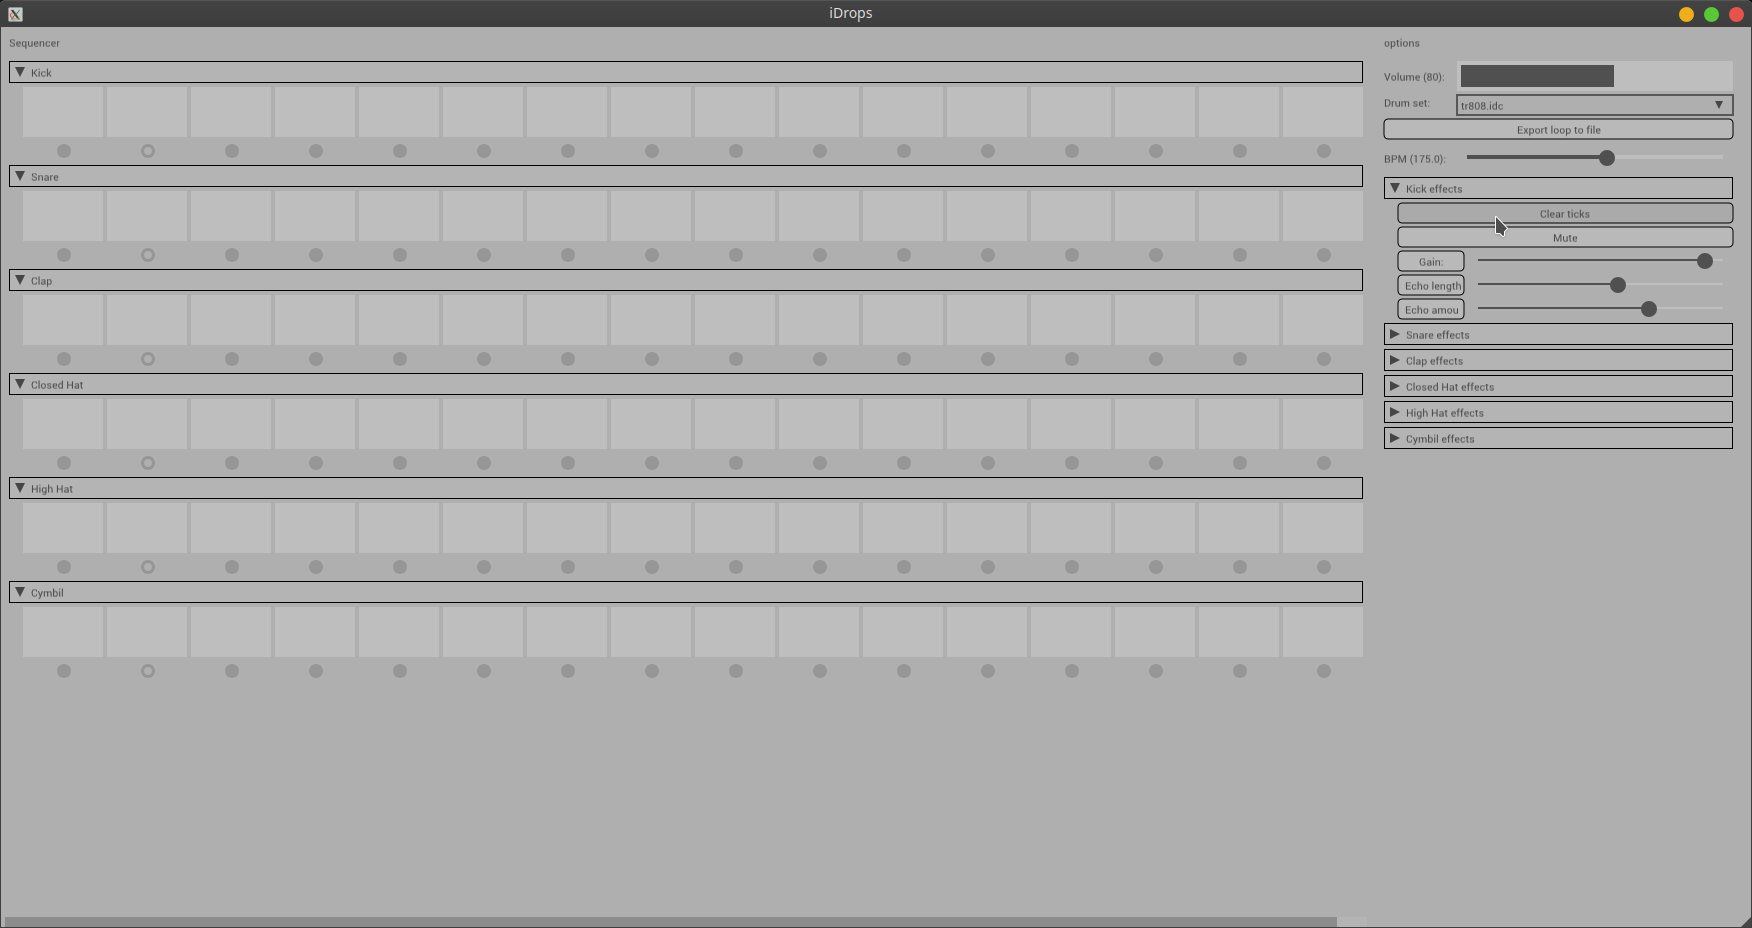
\includegraphics[width=15cm]{./6.png}
\end{center}

Next you are ready to start using more than one instruments. The method is the same,
click the large boxes to toggle an instrument on and off on a specific beat and click
the headers on the options panel to tweak the effects for each instrument.
\begin{center}
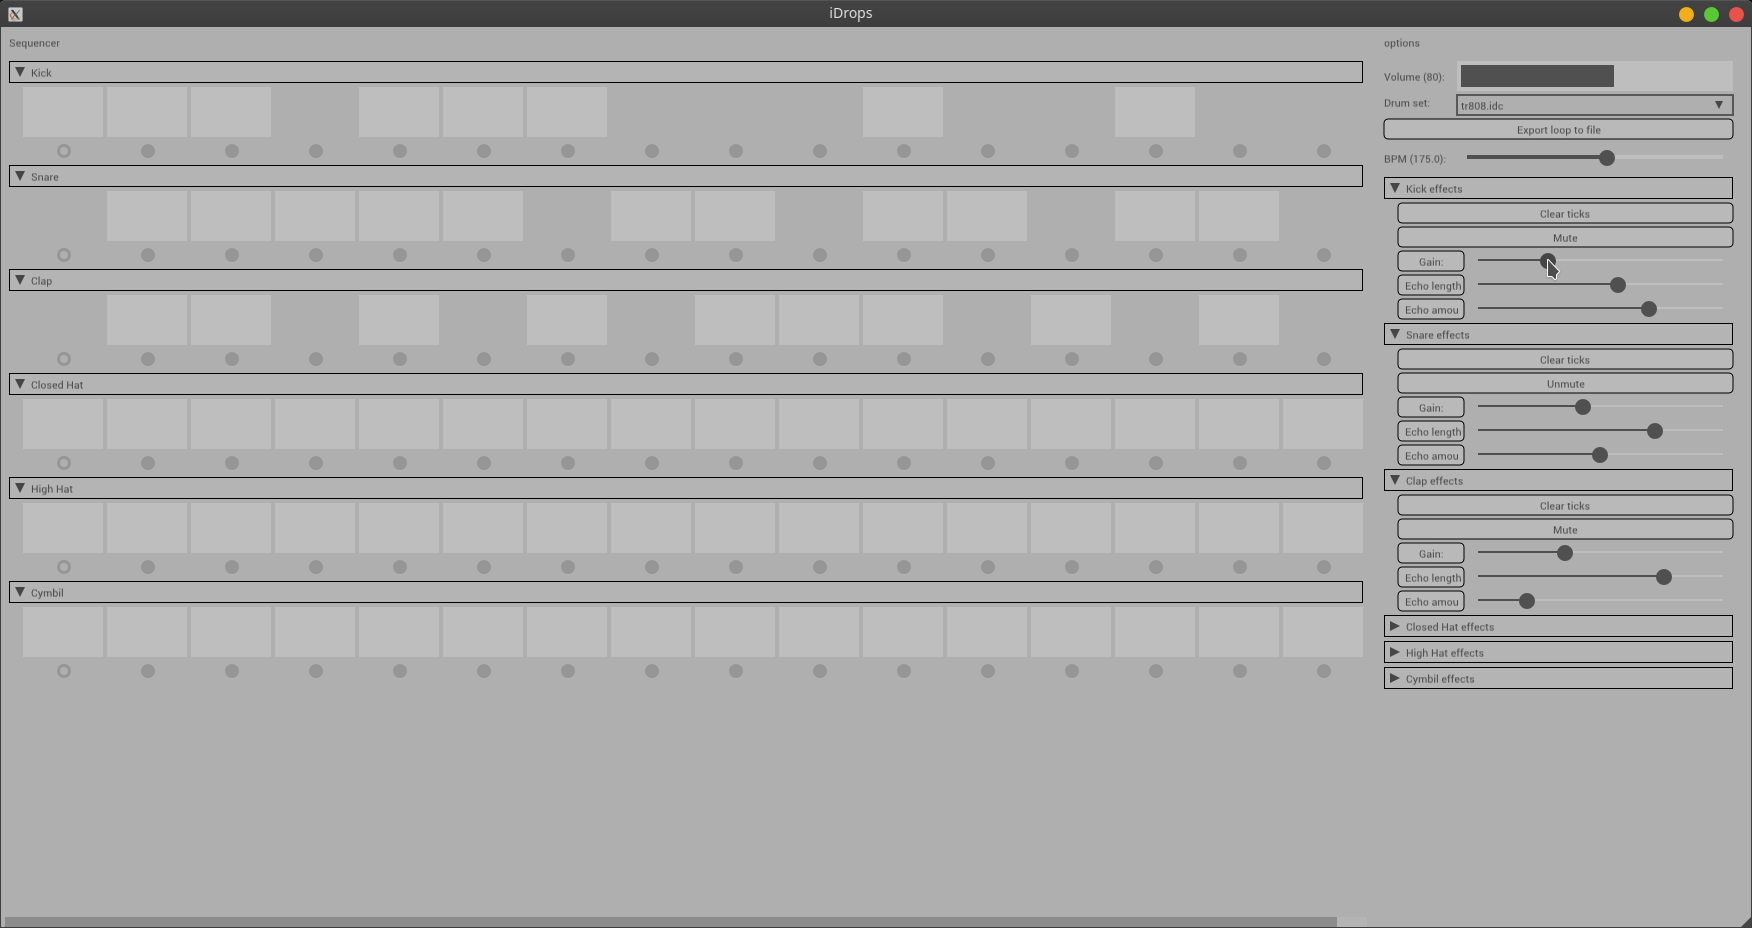
\includegraphics[width=15cm]{./7.png}
\end{center}


At this point things might be a little slow, but don't worry. Use the
slider "bpm" (beats per minute) to adjust the tempo of your drum beat.
The picture below shows the tempo of iDrop being increased.
\begin{center}
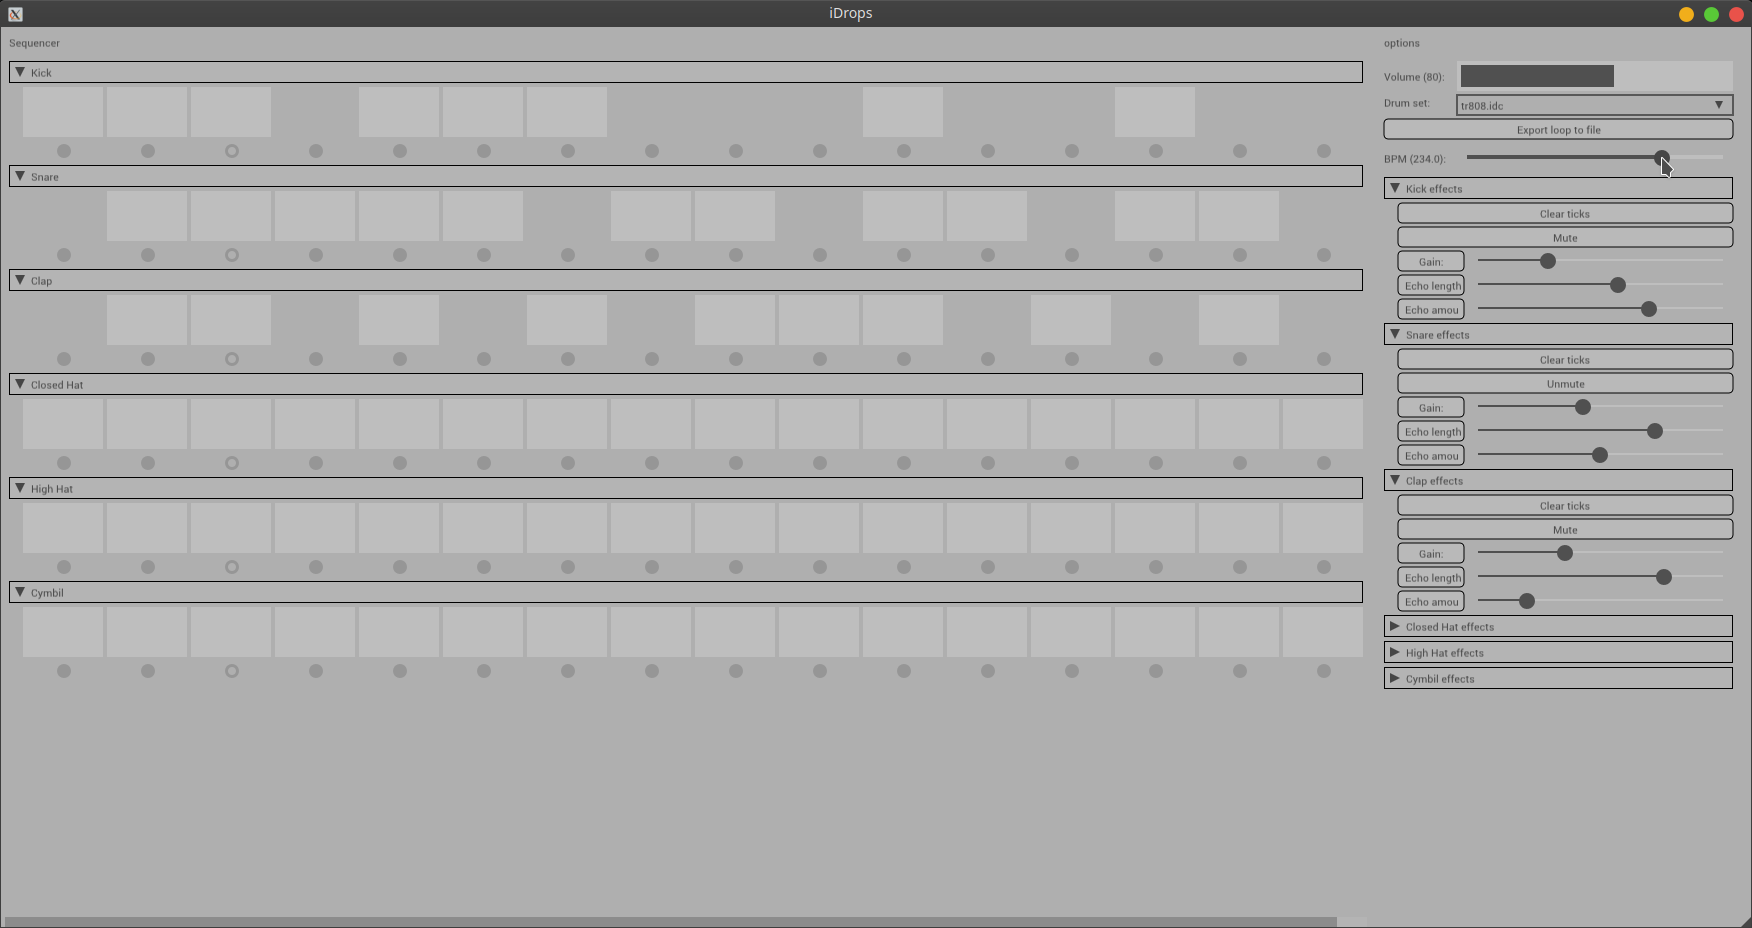
\includegraphics[width=15cm]{./8.png}
\end{center}

Once you are happy with you drum loop hit the "export loop to file" button
on the top right to bring up a dialog box. In this dialog box you can type in
the filename you want to save your loop to and hit "save" to save once you
are ready.

\begin{center}
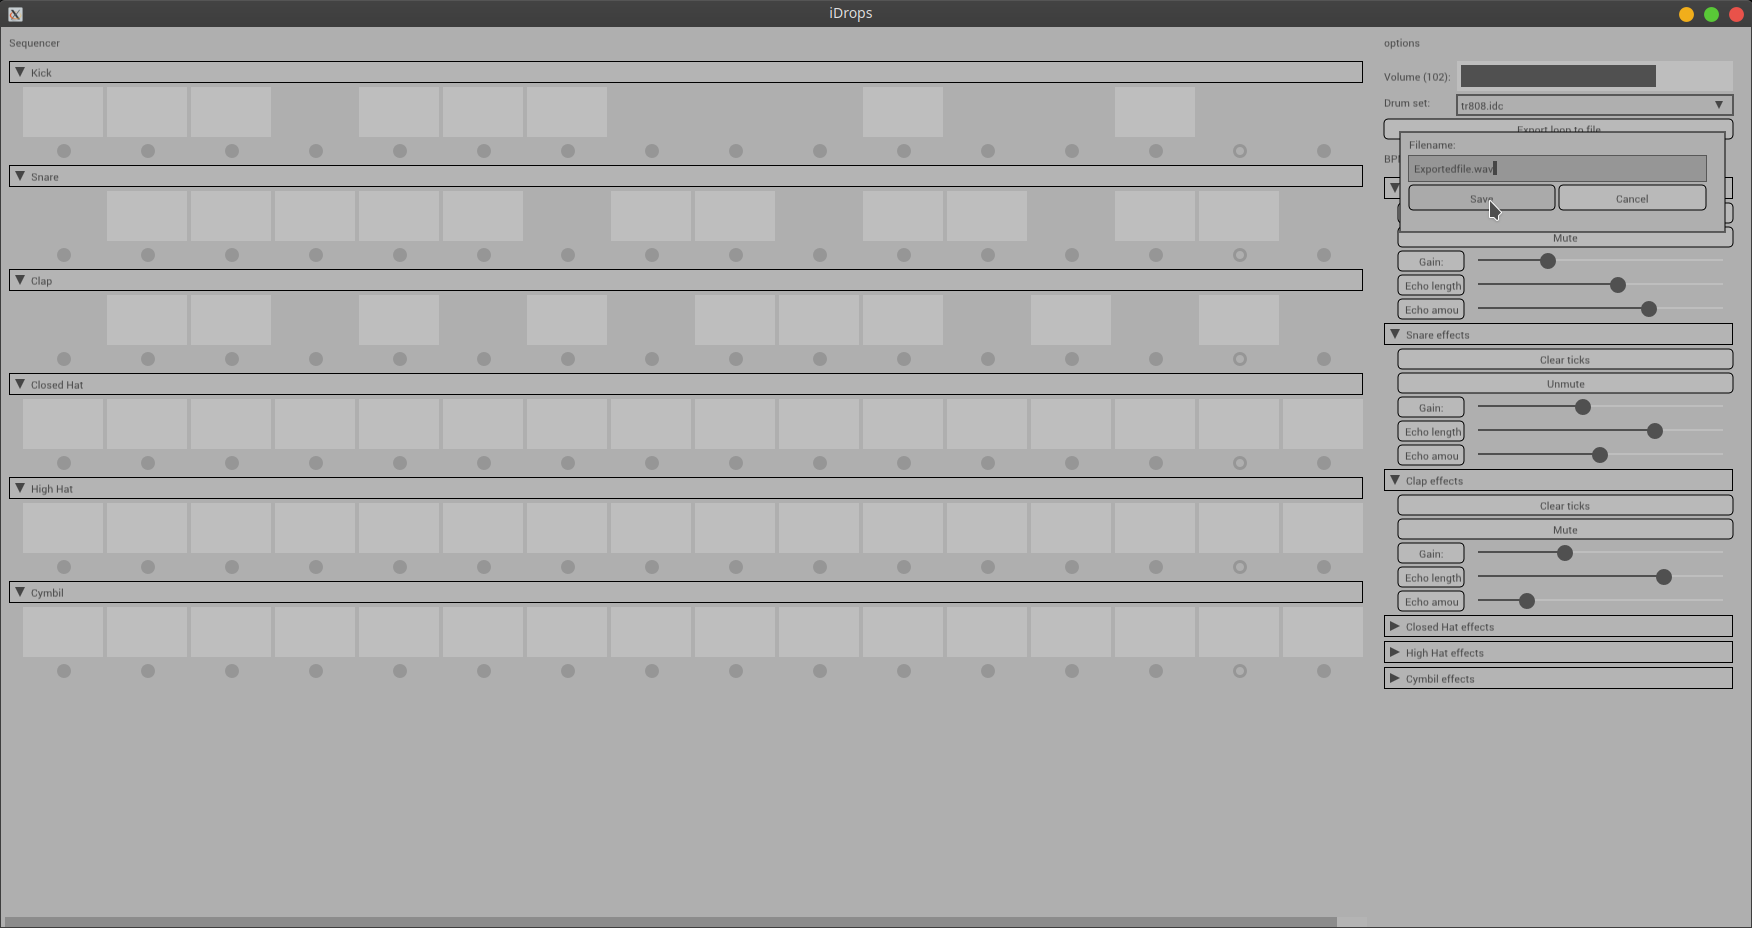
\includegraphics[width=15cm]{./9.png}
\end{center}

\section{Using your own samples}
\label{sec:org962dd45}

Creating your own drum-sets is easy, all you need is a text editor. To start,
create a text file with the name "[DRUM-SET NAME].idc", where [DRUM-SET NAME]
is what you want to name your custom drum-set. Next, open this file in a text 
editor. The format for the .idc file is:

\begin{verbatim}
instrument name 1: "path to file 1" 
instrument name 2: "path to file 2" 
instrument name 3: "path to file 3"
instrument name 4: "path to file 4" 
instrument name 5: "path to file 5" 
\end{verbatim}

The left side of the colon is the name you want to call your instrument in iDrop.
The text in quotes should be a path to the ".wav" file that iDrop will use as the
sample for that instrument. Once you are done writing this file, put the ".idc" file
in the same directory as the iDrop executable and launch iDrop. Navagate to the "drum-set"
drop down on the top right and select your custom drum set from the menu and you are done.

\begin{center}
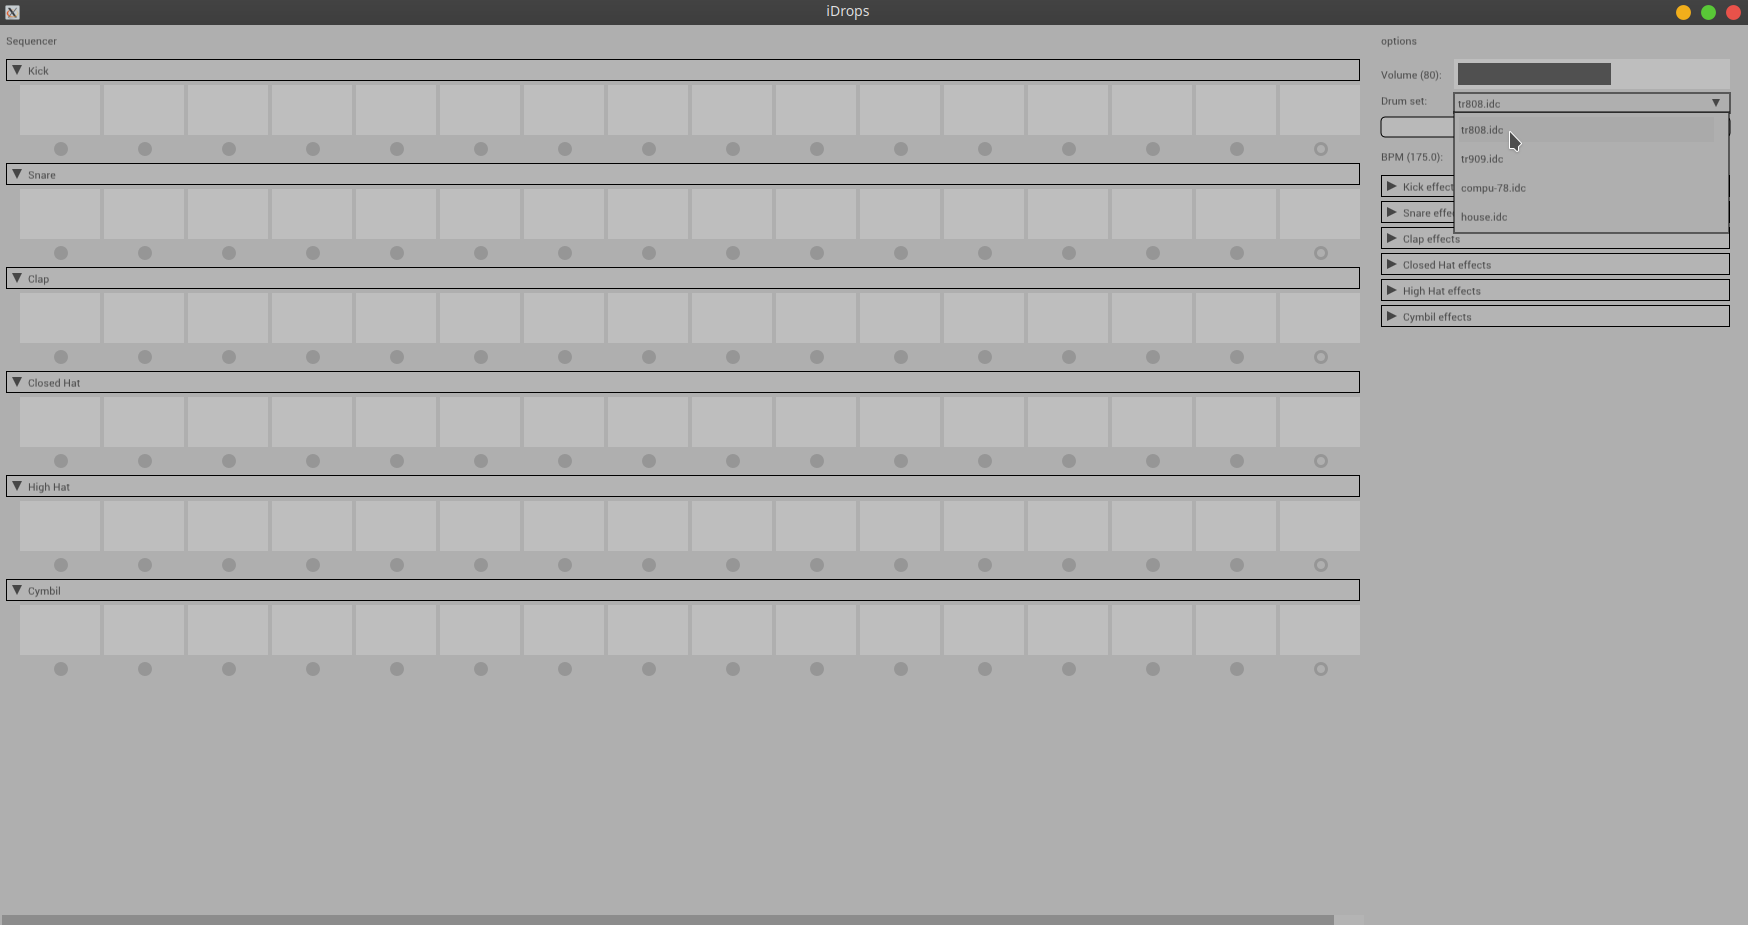
\includegraphics[width=15cm]{./10.png}
\end{center}
\end{document}